\documentclass{article}

\usepackage{changepage}
\usepackage{xcolor}
\usepackage{amsmath}
\usepackage{amssymb}
\usepackage{tikz}
\usepackage{tcolorbox}

\definecolor{blue}{RGB}{0, 166, 223}
\definecolor{lightblue}{RGB}{220, 240, 247}

\newcommand{\definition}[2]{
	\vspace{0.25cm}
	\begin{tcolorbox}[
		colback=lightblue,
		colframe=blue,
		colbacktitle=blue,
		coltitle=white,
		title=\textbf{#1},
		boxrule=0.5pt,
		arc=0pt,
		left=0.4cm,
		right=0.4cm,
		top=0.25cm,
		bottom=0.35cm,
		toptitle=0.1cm,
		bottomtitle=0.075cm
	]
		#2
	\end{tcolorbox}
	\vspace{0.25cm}
}

\newcommand{\theorem}[2]{
	\vspace{0.25cm}
	\begin{tcolorbox}[
		colback=lightblue,
		colframe=blue,
		boxrule=0.5pt,
		toprule=2pt,
		arc=0pt,
		left=0.4cm,
		right=0.4cm,
		top=0.25cm,
		bottom=0.35cm
	]
		\textcolor{blue}{\textbf{Theorem #1}}

		\vspace{0.15cm}

		#2
	\end{tcolorbox}
	\vspace{0.25cm}
}

\newcommand{\header}[1]{
	\vspace{0.25cm}
		\begin{adjustwidth}{0cm}{0cm}
			\textcolor{blue}{\textbf{#1}}
		\end{adjustwidth}
	\vspace{0.25cm}
}

\newcommand{\question}[2]{
	\vspace{0.125cm}
		\begin{adjustwidth}{0.25cm}{0cm}
			\textbf{#1} #2
		\end{adjustwidth}
	\vspace{0.125cm}
}

\newcommand{\container}[1]{
	\vspace{0.25cm}
		\begin{adjustwidth}{0cm}{0cm}
			#1
		\end{adjustwidth}
	\vspace{0.25cm}
}

\newcommand{\solution}[1]{
	\vspace{0.25cm}
		\begin{adjustwidth}{0cm}{0cm}
			\textbf{Solution:} #1
		\end{adjustwidth}
	\vspace{0.25cm}
}

\newcommand{\wrapper}[1]{
	\vspace{0.25cm}
		\begin{adjustwidth}{0cm}{0cm}
			#1
		\end{adjustwidth}
	\vspace{0cm}
}

\newcommand{\calc}[1]{
	\[
		#1
	\]
}

\begin{document}

	\header{2026-10-05}

	\header{Recap}

	\container{
		An r-combination of a finite set X is a subset
		\(Y \subseteq X \) such that N(Y) = r. The symbol
		\(\binom{n}{r}\) denotes the number of r-combinations
		of a set of size n.
	}

	\theorem{9.5.1}{
		For \(n, r \in \mathbb{Z}^{\geq0}, r \leq n, \binom{n}{r} = \frac{n!}{r!(n - r)!}\)
	}

	\header{Example 9.5.6}

	\container{
		Suppose that 2 people (C, D) do not get along and
		cannot be in a team together.

		\calc{Z = \{\text{teams of five without (both C and D)}\}}
		\calc{Y = \{\text{{teams of five}} - \text{{teams of five with both C + D}} \}}
		
		\calc{N(X) = N(Y) - N(Z)\text{, since }Z \subseteq Y}

		\calc{N(Y) = \binom{12}{5} \text{ as above}}
		\calc{N(Z) = \binom{10}{3}}
		\calc{N(X) = \binom{12}{5} - \binom{10}{3} = \boxed{672}}
	}

	\header{Example 9.5.11}

	\container{
		How many ways are there to order the letters in the word \emph{MISSISSIPPI}?

		\wrapper{\textbf{Note:} Since I, S, P are repeated, 11! overcounts.}

		\wrapper{Use the recipe:}

		\begin{adjustwidth}{0.5cm}{0cm}
			\wrapper{(1) Choose 4 out of 11 positions for S \(\to \binom{11}{4}\)}
			\wrapper{(2) Choose 4 out of 7 positions for I \(\to \binom{7}{4}\)}
			\wrapper{(3) Choose 2 out of 3 positions for P \(\to \binom{3}{2}\)}
			\wrapper{(4) Choose 1 out of 1 positions for M \(\to \binom{1}{1}\)}
		\end{adjustwidth}

		\wrapper{Number of orderings: \(\binom{11}{4} \times \binom{7}{4} \times \binom{3}{2} \times \binom{1}{1} = 34,650\)}
	}

	\theorem{9.5.2.}{
		Suppose a set consists of n objects of k different types and
		\(n_i\) objects are of type i and indistinguishable \(\forall i=1,...,k\)
		and \(\sum_{i=1}^{k} n_i = n\). Then the number of distinguishable
		permutations of the n objects is

		\calc{
			\prod_{i=1}^{k} \binom{n - \sum_{j=1}^{i-1} n_j}{n_i} =
			\binom{n}{n_1} \times \binom{n - n_1}{n_2} \times \binom{n-n_1-n_2}{n_3} \times \text{ ... }
		}
		\calc{
			\times \binom{n-n_1-\text{...}-k_{k-1}}{n_k} = \binom{n!}{n_1! \times n_2! \times { ... } \times n_k!}
		}
	}

	\header{9.6 r-combinations with repetition allowed}

	\definition{Definition}{
		A \textbf{multiset} of size r, chosen from a set X of n elements
		is an unordered selection of elements from X with repetition allowed.

		\wrapper{
			For \(X=\{x_1, x_2, \text{ ... }, x_n\}\) we write \(\text{[}x_{i_1}, x_{i_2}, \text{ ... }, x_{i_r}\text{]}\)
			for the multiset, where \(x_{i_j} \in X, \forall j = 1, \text{ ... }, r \text{ and } x_{i_j}\)
			may equal each other.
		}
	}

	\header{Example 9.6.1.}

	\container{Multisets of size 3 chosen from \{1, 2, 3, 4\}:

		\wrapper{
		    \begin{adjustwidth}{0.25cm}{0cm}
			\[
			\begin{aligned}
			    &\text{[1, 1, 1], [1, 1, 2], [1, 1, 3]} \\
			    &\text{[1, 1, 4], [1, 2, 2], [1, 2, 4]} \\
			    &\text{[1, 3, 3], [1, 3, 4], [1, 4, 4]} \\
			    &\text{[2, 2, 2], [2, 2, 3], [2, 2, 4]} \\
			    &\text{[2, 3, 3], [2, 3, 4], [2, 4, 4]} \\
			    &\text{[3, 3, 3], [3, 3, 4], [3, 3, 4]} \\
			    &\text{[3, 4, 4], [4, 4, 4]}
			\end{aligned}
			\]
		    \end{adjustwidth}
		}

		\wrapper{There are 20 multisets of size 3.}
	}

	\container{To do this systematically, use a table:}

	\container{Number of ways of distributing the "x" =
		the number of ways of writing 3 "x" and 3 "", e.g.
		= number of ways of selecting 3 positions of 6 for the
		"x", disregarding the order = \(\binom{6}{3} = 20\)
	}

	\container{
		\begin{center}
			\begin{tabular}{c|c|c|c|c}
				& 1 & 2 & 3 & 4 \\
				\hline
				\text{[1, 1, 1]} & xxx & & & \\
				\text{[1, 1, 2]} & xx & x & & \\
				\text{[2, 4, 4]} & & x & & xx
			\end{tabular}
		\end{center}
	}

	\theorem{9.6.1}{
		The number of multisets of size r chosen from n elements is

		\calc{\binom{n + r - 1}{r}}
	}

	\header{Example 9.6.2}

	\container{
		Select 15 cans of softdrinks from a menu of 5.
		Each selection corresponds to a multiset of size
		15 from a set of 5. Hence, there are

		\calc{\binom{15+5-1}{15} = 3,876 \text{ possibilities}}
	}

	\header{Example 9.6.5}

	\container{
		How many sol's are there to
		\(x_1 + x_2 + x_3 + x_4 = 10\) if \(x_i \in \mathbb{Z}^{+}
		\forall i = 1, 2, 3, 4\)

		\wrapper{
			Think about 4 categories \(x_1, \text{ ... }, x_4\),
			from which we select 10 units:
		}

		\wrapper{
			\begin{center}
				\begin{tabular}{c|c|c|c|c}
					& \(x_1\) & \(x_2\) & \(x_3\) & \(x_4\) \\
					\hline
					& xxxxxxx & x & x & x \\
					& xxxx & xxx & xx & x \\
					& x & x & x & xxxxxxx
				\end{tabular}
			\end{center}
		}

		\wrapper{
			Hence, there are

			\calc{\binom{10+4-1}{10} = 286 \text{ sol's}}
		}
	}

	\container{
		Summary of formulas when choosing k elements from n:
	}

	\container{
		\begin{center}
			\renewcommand{\arraystretch}{1.5}
			\setlength{\tabcolsep}{12pt}

			\begin{tabular}{c|c|c}
				& \textbf{Order matters} & \textbf{Order doesn't matter} \\
				\hline
				\textbf{Repetition allowed}
					& \(n^k\)
					& \(\binom{n+k-1}{k}\) \\
				\textbf{Repetition not allowed}
					& \(P(n,k)\)
					& \(\binom{n}{k}\)
			\end{tabular}
		\end{center}
	}

	\header{10.1 Trails, Paths and Circuits}

	\container{
		\begin{center}
			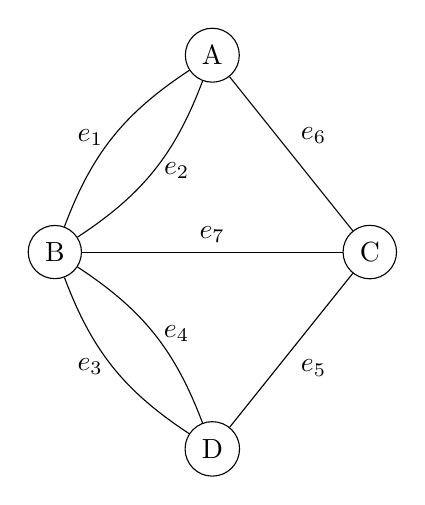
\begin{tikzpicture}[
				vertex/.style={
					circle,
					draw=black,
					fill=white,
					minimum size=0.65cm
				},
				edge/.style={
					draw=black
				}
			]

				\node[vertex] (A) at (0,2.5) {A};
				\node[vertex] (B) at (-2,0) {B};
				\node[vertex] (C) at (2,0) {C};
				\node[vertex] (D) at (0,-2.5) {D};

				\draw[edge, bend right=18]
					(A) to node[left] {\(e_1\)} (B);

				\draw[edge, bend left=18]
					(A) to node[right] {\(e_2\)} (B);

				\draw[edge, bend right=18]
					(B) to node[left] {\(e_3\)} (D);

				\draw[edge, bend left=18]
					(B) to node[right] {\(e_4\)} (D);

				\draw[edge]
					(A) to node[above right] {\(e_6\)} (C);

				\draw[edge]
					(B) to node[above] {\(e_7\)} (C);

				\draw[edge]
					(D) to node[below right] {\(e_5\)} (C);

			\end{tikzpicture}
		\end{center}
	}
	
	\definition{Definition (1.4)}{
		A graph G consists of two finite sets and a function:

		\wrapper{
			\(V(G) \neq \emptyset\), the set of \textbf{vertices}

			\(E(G)\), the set of \textbf{edges}

			\(\phi_G : E(G) \to \{\{x, y\} \mid x,y \in V(G)\}\), the \textbf{incidence function}
		}

		\wrapper{
			If \(\phi_G(e) = \{x, y\}\), e is said to connect x and y
		}

		\wrapper{
			If \(\phi_G(e) = \{x\}\), e is a loop.
		}

		\wrapper{
			Two vertices which are connected are called \textbf{adjacent}
			and a vertex not connected to any edge is called \textbf{isolated}.
		}

		\wrapper{
			The number of edges connected to a vertex is its degree, deg(v).
			A loop is counted twice.
		}
	}
\end{document}
